\documentclass[12pt]{article}
\usepackage[utf8]{inputenc}
\usepackage[russian]{babel}
\usepackage{amsmath}
\usepackage{amssymb}
\usepackage{amsfonts}
\usepackage{graphicx}
\usepackage{epstopdf}

\title{Draft}

\begin{document}
\maketitle

\newcommand{\sn}{\textrm{sn}}
\newcommand{\cn}{\textrm{cn}}
\newcommand{\dn}{\textrm{dn}}
\newcommand{\sd}{\textrm{sd}}
\newcommand{\cd}{\textrm{cd}}
\newcommand{\nd}{\textrm{nd}}
\newcommand{\am}{\textrm{am}}

\subsection*{Модель}

Рассматривается безразмерная версия GPE:
%
\begin{equation}
i \dfrac{\partial \psi}{\partial t} = -\dfrac{1}{2} \dfrac{\partial^2 \psi}{\partial x^2} + U(x) \psi + g |\psi|^2 \psi.
\label{eq:GPE} 
\end{equation}
%
Здесь $\int |\psi|^2 dx = N$, где $N$ -- число атомов.
Потенциал имеет вид $U(x) = h ((x/x_0)^2 - 1)^2$ (или, возможно, другой симметричный double-well потенциал).
Гаильтониан этого уравнения выглядит следующим образом:
%
\begin{equation}
H = \int \Big\{ -\dfrac{1}{2} \psi^\dag \dfrac{d^2 \psi}{dx^2} + \psi^\dag \psi U(x) + \dfrac{g}{2} \psi^{\dag 2} \psi^2  \Big\} dx.
\label{eq:gpe_hamiltonian}
\end{equation}
%

В этой задаче изучается двухмодовое приближение
%
\begin{equation}
\psi = \psi_1(t) \Phi_1(x) + \psi_2(t) \Phi_2(x),
\label{eq:two_modes}
\end{equation}
%
где
%
\begin{equation}
\Phi_{1,2} = \dfrac{\Phi_+ \pm \Phi_-}{\sqrt{2}}, \quad \Phi_{\pm}(x) = \pm \Phi_{\pm} (-x),
\label{eq:conditions}
\end{equation}
%
а моды $\Phi_{\pm}$ удовлетворяют стационарному уравнению
%
\begin{equation}
\beta_{\pm} \Phi_{\pm} = -\dfrac{1}{2} \dfrac{d^2 \Phi_{\pm}}{dx^2} + U(x) \Phi_{\pm} + g \Phi_{\pm}^3.
\label{eq:stationary}
\end{equation}
%
Полагаем, что для $\Phi_{\pm}$ выполняется условие нормировки $\int \Phi_{\pm}^2 dx = 1$, а значит, что и $\int \Phi_{1,2}^2 dx = 1$.
Также $\int |\psi|^2 dx = \int |\psi_1 \Phi_1 + \psi_2 \Phi_2|^2 = |\psi_1|^2 + |\psi_2|^2 = N$.
Теперь подставим выражение (\ref{eq:two_modes}) в гамильтониан (\ref{eq:gpe_hamiltonian}) и проинтегрируем.
Выражение для гамильтониана принимает вид:
%
\begin{eqnarray*}
\hat{H} & = & (\psi_1^\dag \psi_1 + \psi_2^\dag \psi_2) \Big[ \dfrac{1}{4} \int (\Phi_+')^2 + (\Phi_-')^2  dx + \dfrac{1}{2} \int ((\Phi_+)^2 + (\Phi_-)^2) U(x) dx \Big] \\[10pt]
&& +(\psi_1^\dag \psi_2 + \psi_2^\dag \psi_1) \Big[ \dfrac{1}{4} \int (\Phi_+')^2 - (\Phi_-')^2 dx + \dfrac{1}{2} \int ((\Phi_+)^2 - (\Phi_-)^2)U(x) dx \Big] \\[10pt]
&& +\dfrac{1}{2} \Big[ \psi_1^{\dag 2} \psi_1^2 \dfrac{1}{4} (\gamma_{++} + \gamma_{--} + 6 \gamma_{+-}) + \psi_2^{\dag 2} \psi_2^2 \dfrac{1}{4}(\gamma_{++} + \gamma_{--} + 6 \gamma_{+-})  \\[10pt]
&& +(\psi_1^{\dag 2} \psi_1 \psi_2 + \psi_1^\dag \psi_1^2 \psi_2^\dag) \dfrac{1}{2}(\gamma_{++} - \gamma_{--}) + (\psi_1^\dag \psi_2^\dag \psi_2^2 + \psi_2^{\dag 2} \psi_2 \psi_1) \dfrac{1}{2} (\gamma_{++} - \gamma_{--})\\[10pt]
&& + (\psi_1^{\dag 2} \psi_2^2 + 4 \psi_1^\dag \psi_1 \psi_2^\dag \psi_2 + \psi_1^2 \psi_2^{\dag 2}) \dfrac{1}{4} (\gamma_{++} - 2 \gamma_{+-} + \gamma_{--}) \Big].
\end{eqnarray*}
%
Будем использовать следующие обозначения:
%
\begin{equation}
\begin{array}{c}
	\gamma_{ij} = g \int \Phi_i^2 \Phi_j^2 dx, \quad i,j \in \{+,-\}; \\[10pt]
	\quad A = \dfrac{\gamma_{++} + \gamma_{--} + 6 \gamma_{+-}}{4}; \quad E = \dfrac{\gamma_{++} - \gamma_{--}}{2}; \\[10pt]
	C = \dfrac{\gamma_{++} + \gamma_{--} - 2\gamma_{+-}}{4}; \\[10pt]
	G = \dfrac{1}{2} \int (\Phi_+')^2 - (\Phi_-')^2 dx + \int ((\Phi_+)^2 - (\Phi_-)^2)U(x) dx.
\end{array}
\label{eq:subs}
\end{equation}
%
Заметим, что $G$ можно выразить по-другому, используя уравнения для стационарных состояний (\ref{eq:stationary}):
%
\begin{equation}
G = \beta_+ - \beta_- - 2E;
\end{equation}
%

Перепишем гамиьльтониан в новых обозначениях, избавившись от первого слагаемого, которое является постоянной ($\psi_1^\dag \psi_1 + \psi_2^\dag \psi_2 \equiv N$).
%
\begin{equation}
\begin{array}{lcl}
	\hat{H} & = & \dfrac{G}{2} (\psi_1^\dag \psi_2 +  \psi_1 \psi_2^\dag) + \dfrac{A}{2} (\psi_1^{\dag 2} \psi_1^2 + \psi_2^{\dag 2} \psi_2^2) \\[10pt]
	& & +\dfrac{E}{2} (\psi_1^{\dag 2} \psi_1 \psi_2 + \psi_1^\dag \psi_1^2 \psi_2^\dag + \psi_1^\dag \psi_2^\dag \psi_2^2 + \psi_1 \psi_2^{\dag 2} \psi_2) \\[10pt]
	& & +\dfrac{C}{2} (\psi_1^{\dag 2} \psi_2^2 + 4 \psi_1^\dag \psi_1 \psi_2^\dag \psi_2 + \psi_1^2 \psi_2^{\dag 2}).
\end{array}
\label{eq:hamiltonian}
\end{equation}
%

Из этого гамильтониана через уравнения Гейзенберга может быть получена система уравнений, так называемая I2M модель:
%
\begin{equation}
\begin{array}{lcl}
	i \psi_{1,t} & = & (A |\psi_1|^2 + 2C |\psi_2|^2 + \dfrac{E}{2} \psi_1 \psi_2^*) \psi_1 + \\[10pt]
	&& + (\dfrac{G}{2} + E |\psi_1|^2 + \dfrac{E}{2} |\psi_2|^2 + C \psi_1^* \psi_2) \psi_2; \\[10pt]
	i \psi_{2,t} & = & (A |\psi_2|^2 + 2C |\psi_1|^2 + \dfrac{E}{2} \psi_2 \psi_1^*) \psi_2 + \\[10pt] 
	&& + (\dfrac{G}{2} + E |\psi_2|^2 + \dfrac{E}{2}|\psi_1|^2 + C \psi_2^* \psi_1) \psi_1.
\end{array}
\label{eq:I2M}
\end{equation}
%

Воспользовавшись нормировкой, полученную систему можно упростить, сделав ее, тем самым, похожей на модель из статьи Ananikian, Bergeman.
%
\begin{equation*}
\begin{array}{c}
	i \psi_{1,t} = ((A - 2C) |\psi_1|^2 + \dfrac{E}{2} \psi_1 \psi_2^*) \psi_1 + (\dfrac{G}{2} + \dfrac{EN}{2} + \dfrac{E}{2} |\psi_1|^2 + C \psi_1^* \psi_2) \psi_2; \\[10pt]
	i \psi_{2,t} = ((A - 2C) |\psi_2|^2 + \dfrac{E}{2} \psi_2 \psi_1^*) \psi_2 + (\dfrac{G}{2} + \dfrac{EN}{2} + \dfrac{E}{2} |\psi_2|^2 + C \psi_2^* \psi_1) \psi_1.
\end{array}
\end{equation*}
%

\subsection*{Переход к операторам спина}

В выражении для гамильтониана перейдем к операторам $S_0$, $S_x$, $S_y$, $S_z$, определенных следующим образом:
%
\begin{equation}
\begin{array}{c}
	S_0 = \dfrac{1}{2} (\psi_1^\dag \psi_1 + \psi_2^\dag \psi_2), \quad S_z = \dfrac{1}{2} (\psi_2^\dag \psi_2 - \psi_1^\dag \psi_1), \\[10pt]
	S_x = \dfrac{1}{2} (\psi_1^\dag \psi_2 + \psi_1 \psi_2^\dag), \quad S_y = \dfrac{i}{2} (\psi_1^\dag \psi_2 - \psi_1 \psi_2^\dag), \\[10pt]
	S_+ = \psi_1 \psi_2^\dag, \quad S_- = \psi_1^\dag \psi_2, \quad S_{\pm} = S_x \pm iS_y.
\end{array}
\end{equation}
%
Выполняется тождество:
%
\begin{equation}
S_0^2 + S_x^2 + S_y^2 + S_z^2 = \dfrac{1}{2}(N^2 + N) = Const.
\label{eq:sum_of_squares}
\end{equation}
%
Тогда
%
\begin{eqnarray*}
&& \psi_1^\dag \psi_2 + \psi_1 \psi_2^\dag = 2S_x; \\
&& \psi_1^{\dag 2} \psi_1^2 + \psi_2^{\dag 2} \psi_2^2 = 2(S_0^2 + S_z^2 - S_0); \\
&& \psi_1^{\dag 2} \psi_1 \psi_2 + \psi_1^\dag \psi_1^2 \psi_2^\dag + \psi_1^\dag \psi_2^\dag \psi_2^2 + \psi_1 \psi_2^{\dag 2} \psi_2 = 2(2S_0 - 1) S_x; \\
&& \psi_1^{\dag 2} \psi_2^2 + 4 \psi_1^\dag \psi_1 \psi_2^\dag \psi_2 + \psi_1^2 \psi_2^{\dag 2} = S_-^2 + S_+^2 + 4(S_0^2 - S_z^2).
\end{eqnarray*}
%
%
$$\hat{H} = G S_x + A(S_z^2 + S_0^2 - S_0) + E(2S_0 - 1) S_x + C(S_x^2 - S_y^2 + S_0^2 - 2S_z^2).$$
%
В полученном выражении выразим $S_y^2$ через $S_z^2$ и $S_x^2$ (см. выражение (\ref{eq:sum_of_squares}) и отбросим все постоянные.
%
$$\hat{H} = G S_x + A S_z^2 + E(2S_0 - 1) S_x + C(2 S_x^2 - S_z^2).$$
%
Заметим, что $A - C = 2 \gamma_{+-} = \alpha > 0$, также $2S_0 = N \gg 1$; $2C = \beta$; $EN+G = B$.
Приходим к следующему выражению для гамильтониана:
%
\begin{equation}
\hat{H} = \alpha S_z^2 + \beta S_x^2 + B S_x.
\label{eq:spin_hamiltonian}
\end{equation}

\subsection*{Дифференциальное представление операторов}

В выражении (\ref{eq:spin_hamiltonian}) перейдем к дифференциальному представлению операторов:
%
\begin{equation}
S_z = -i \dfrac{d}{d \phi}, \quad S_x = S \cos \phi - \sin \phi \dfrac{d}{d \phi}, \quad S_y = S \sin \phi + \cos \phi \dfrac{d}{d \phi}.
\label{eq:diff_repr}
\end{equation}
%
Должны выполняться следующие коммутационные соотношения:
%
$$[S_x, S_y] = iS_z, \quad [S_z, S_x] = iS_y, \quad [S_y, S_z] = iS_x.$$
%
Заметим, что
%
\begin{equation}
\begin{array}{lcl}
	S_x^2 & = & (S \cos \phi - \sin \phi \dfrac{d}{d \phi})^2 = \\
	& = & S^2 \cos^2 \phi + S \sin^2 \phi + (\frac{1}{2} - S) \sin 2 \phi \dfrac{d}{d \phi} + \sin^2 \phi \dfrac{d^2}{d \phi^2}.
\end{array}
\end{equation}
%
Выражение для Гамильтониана после некоторых преобразований и отбрасывания постоянных принимает вид:
%
\begin{equation*}
\begin{array}{lcl}
	\hat{H} & = & -(\alpha - \beta \sin^2 \phi) \dfrac{d^2}{d \phi^2} - (B \sin \phi + \beta (S - \frac{1}{2}) \sin 2 \phi) \dfrac{d}{d \phi} \\[10pt]
	&& + BS \cos \phi - \beta S^2 \sin^2 \phi - \beta S \cos^2 \phi.
\end{array}
\end{equation*}
%
Поставим задачу на собственные значения и собственные функции гамильтониана в дифференциальной форме:
%
\begin{equation}
\hat{H} \Phi = E \Phi.
\end{equation}
%
\begin{equation}
\begin{array}{l}
	(\alpha - \beta \sin^2 \phi) \dfrac{d^2 \Phi}{d \phi^2} + (B \sin \phi + \beta (S - \frac{1}{2}) \sin 2\phi) \dfrac{d \Phi}{d \phi} \\[10pt]
	+ (E - BS \cos \phi + \beta S^2 \sin^2 \phi + \beta S \cos^2 \phi) = 0.
\end{array}
\end{equation}

\subsection*{Замена переменных}

Избавимся от переодической зависимости при второй производной с помощью замены $\phi \to x$,
%
\begin{equation*}
x = \int \limits_0^\phi \dfrac{d \phi'}{\sqrt{1 - \frac{\beta}{\alpha} \sin^2 \phi'}} = F(\phi, \sqrt{\beta / \alpha}),
\end{equation*}
%
где $F(\phi, \sqrt{\beta / \alpha})$ -- неполный эллиптический интеграл первого рода.
При таком преобразовании
%
\begin{eqnarray*}
\dfrac{d}{d \phi} & = & \dfrac{dx}{d \phi} \dfrac{d}{dx} =  \dfrac{1}{(1 - \frac{\beta}{\alpha} \sin^2 \phi)^{1/2}} \dfrac{d}{dx};\\
\dfrac{d^2}{d \phi^2} & = & \left( \dfrac{dx}{d\phi} \right)^2 \dfrac{d^2}{dx^2} + \left( \dfrac{d^2 x}{d \phi^2} \right) \dfrac{d}{dx} = \\
& = & \dfrac{1}{1 - \frac{\beta}{\alpha} \sin^2 \phi} \dfrac{d^2}{dx^2} + \dfrac{\frac{\beta}{\alpha} \sin \phi \cos \phi}{(1 - \frac{\beta}{\alpha} \sin^2 \phi)^{3/2}} \dfrac{d}{dx}.
\end{eqnarray*}
%
Далее, тригонометричекие функции перейдут в свои эллиптические аналоги: $\sin \phi = \sn x$, $\cos \phi = \cn x$, $1 - \frac{\beta}{\alpha} \sn^2 x = \dn^2 x$.
%
\begin{equation}
\begin{array}{l}
	\alpha \dfrac{d^2 \Phi}{d x^2} + \dfrac{B~\sn x + 2 \beta S~\sn x~\cn x}{\dn x} \dfrac{d \Phi}{dx} \\[10pt]
	+ (E - BS~\cn x + \beta S^2~\sn^2 x + \beta S~\cn^2 x) \Phi = 0.
\end{array}
\end{equation}
%
Далее избавимся от первой производной таким образом: $\Phi = \Psi e^{f(x)}$, где $f(x)$ -- некоторая пока неизвестная функция.
При таком преобразовании:
%
\begin{equation*}
\begin{array}{lcl}
	\dfrac{d}{dx} & \to & \dfrac{d}{dx} + f';\\[10pt]
	\dfrac{d^2}{dx^2} & \to & \dfrac{d^2}{dx^2} + 2f' \dfrac{d}{dx} + f'' + (f')^2.
\end{array}
\end{equation*}
%
Коэффициент при первой производной $d/dx$ обращается в ноль при следующем условии на функцю $f$:
%
\begin{equation}
f' = -\dfrac{B~\sn x + 2 \beta S~\sn x~\cn x}{2 \alpha~\dn x}.
\label{eq:f_condition}
\end{equation}
%
Можно проверить (я проверил), что
%
\begin{equation}
f = S \ln~\dn x + \frac{B}{2 \sqrt{\beta(\alpha - \beta)}} \arctan \left( \sqrt{\frac{\beta}{\alpha - \beta}}~\cn x \right)
\end{equation}
%
удовлетворяет условию (\ref{eq:f_condition}).
Выражение для второй производной:
%
$$f'' = -\frac{1}{2 \alpha} \left( B~\cn x + 2\beta S (\cn^2 x - \sn^2 x) + \frac{\beta B~\sn^2 x~\cn x + 2 \beta^2 S~\sn^2 x~\cn^2 x}{\alpha~\dn^2 x} \right).$$
%
Приходим к следующему уранению:
%
\begin{equation}
\alpha \frac{d^2 \Psi}{dx^2} + (E - V(x)) \Psi = 0,
\label{eq:shrod1}
\end{equation}
%
с потенциалом
%
\begin{equation}
V(x) = \frac{(\frac{1}{4}B^2 - \beta(\alpha - \beta) S (S+1))~\sn^2 x + \alpha B (S + \frac{1}{2})~\cn x}{\alpha~\dn^2 x}.
\end{equation}
%
Введем обозначения $\Lambda = \frac{G}{\alpha S}$, $\lambda = \beta / \alpha$.
Далее полагаем, что $E = 0$, $B = EN + G = G$, $S = N/2 \gg 1$, тогда уравнение (\ref{eq:shrod1}) можно переписать в виде
%
\begin{equation}
\frac{d^2 \Psi}{dx^2} + (E - S^2 V(x)) \Psi = 0,
\label{eq:shrod2}
\end{equation}
% 
где
%
\begin{equation}
V(x) = \frac{(\frac{1}{4} \Lambda^2 - \lambda (1 - \lambda))~\sn^2 x + \Lambda~\cn x}{\dn^2 x}.
\end{equation}
%
Линейное преобразование пространственной координаты: $\phi \to \phi + \pi$, $x \to x + 2K(\lambda)$, потенциал изменится на
%
\begin{equation}
V(x) = \frac{(\frac{1}{4} \Lambda^2 - \lambda (1 - \lambda))~\sn^2 x - \Lambda~\cn x}{\dn^2 x}.
\end{equation}
%
Построим графики $V(x)$ для различных значений параметров $\Lambda$, $\lambda$.
%
\begin{figure}[Ht!]
\center{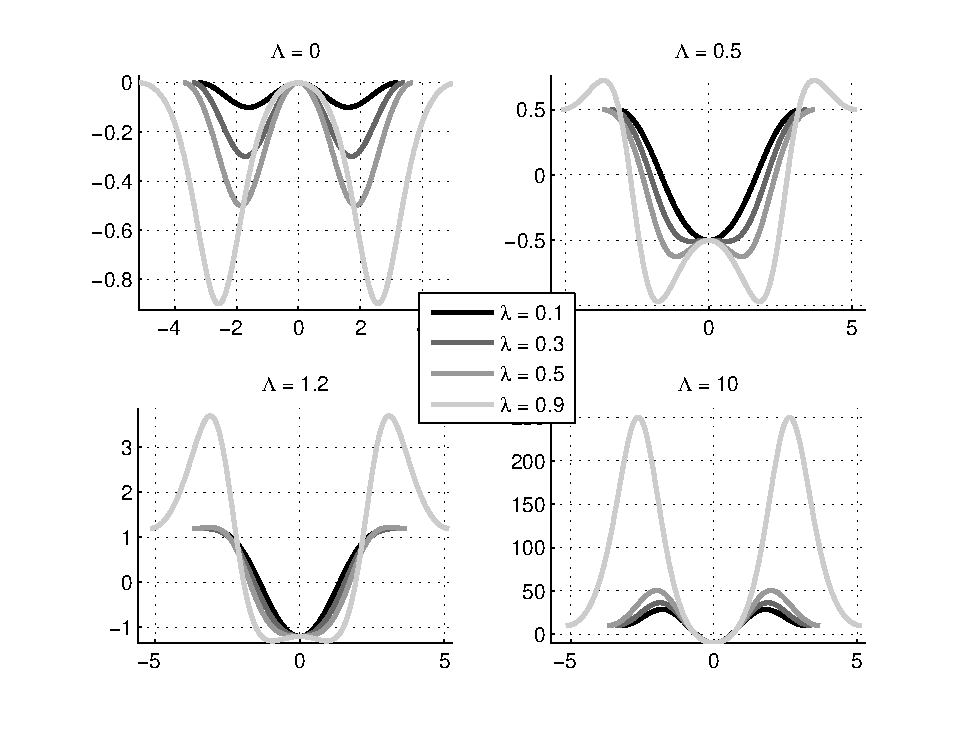
\includegraphics[width=1\linewidth]{pic/V_1period_shifted.eps}}
\caption{$V(x)$ на 1-ом периоде функций Якоби ($[-2K; 2K]$) после сдвига}
\end{figure}
%
%\begin{figure}[Ht!]
%\center{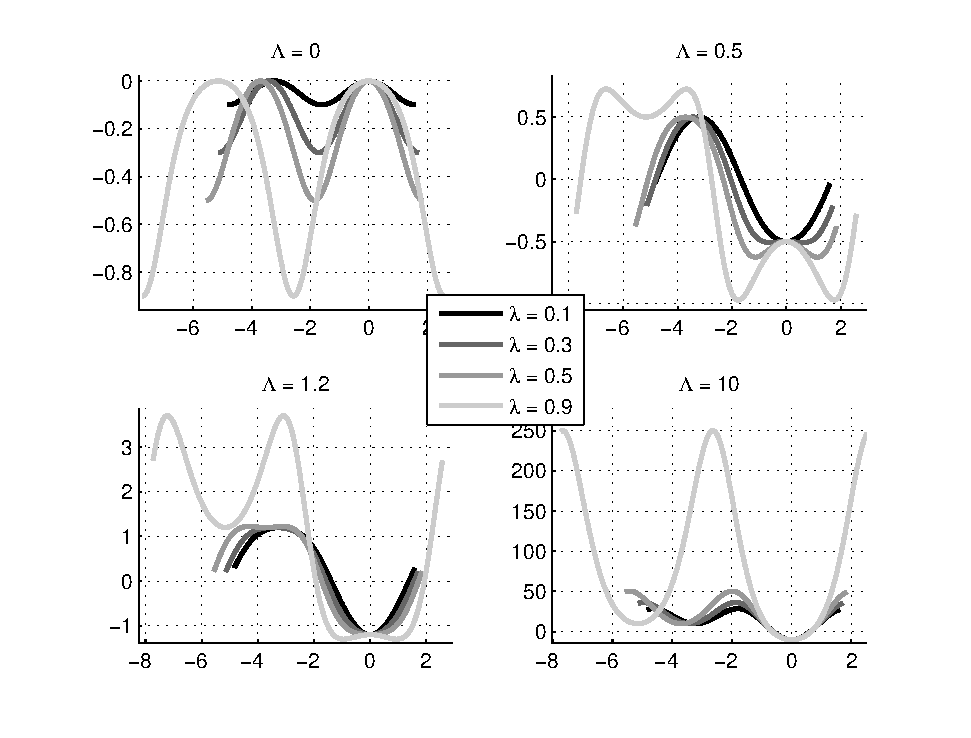
\includegraphics[width=1\linewidth]{pic/V_1period_shifted_asym.eps}}
%\caption{На 1-ом периоде функций Якоби ($[-3K; K]$)}
%\end{figure}
%

\subsection*{Фазовый переход в задаче о туннелировании}

Рассмотрим уравнение Ньютона:
%
\begin{equation}
\frac{1}{2} \dot{x}^2 = S^2 V(x) - E.
\end{equation}
%
Тип фазового перехода определяется зависимостью периода колебаний термона от энергии $\tau(E)$.
Если $\tau(E)$ монотонная (монотонно-убывающая), имеет место фазовый переход 1-го рода, а иначе, когда зависимость $\tau(E)$ немонотонная, фазовый переход 2-го рода.

\paragraph{Fock: $\Lambda = 0$.}
Выражение для потенциала:
%
\begin{equation}
V_F (x) = -\lambda (1 - \lambda)~\sd^2 x.
\end{equation}
%
Типичный график потенциала показан на Рис. \ref{pic:potential_fock}
%
\begin{figure}[Ht!]
\center{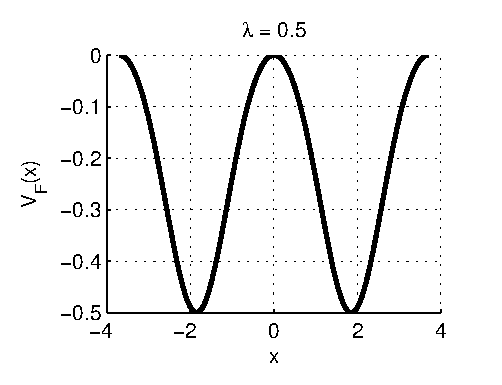
\includegraphics[width=0.5\linewidth]{pic/V_Fock.eps}}
\caption{$V_F (x)$ на 1-ом периоде функций Якоби ($[-2K; 2K]$) после сдвига, $\lambda = 0.5$}
\label{pic:potential_fock}
\end{figure}
%
Используем критерий фазового перехода из статьи Чудновского в PRL.
Разложим $V(x)$ в нуле в ряд тейлора:
%
\begin{equation}
V_F (x) = -\lambda (1 - \lambda) (2x^2 - 8(1 - 2\lambda)x^4 + o(x^4)).
\end{equation}
%

\textbf{Утверждение.} Знак перед 4-й степенью оперделяет локальное поведение $\tau(E)$ вблизи точки $E_0$ исчезнования термона.
Знаку ``$+$'' соответствует убывание периода в окрестности $E_0$, а знаку ``$-$'' -- возрастание.
Это означает, что в случае ``$-$'' имеет место фазовый переход 1-го рода.
Случай ``$+$'' не означает, что функция $\tau(E)$ монотонна, однако мы, вслед за работой Чудновского, будем полагать ее в этом случае монотонной (т.е. что ее локальное поведение можно экстраполировать на глобальное), что влечет а собой фазовый переход 2-го рода.

Результат: при $\lambda < 0.5$ имеет место фазовый переход 2-го рода, при $\lambda > 0.5$ -- 1-го рода.
Этот результат согласуется с численным счетом.
%
\begin{figure}[Ht!]
\center{\includegraphics[width=1\linewidth]{pic/tau_on_E_Fock.eps}}
\caption{$\tau(E)$, Fock, {\bf qualitative only!}}
\end{figure}
%

\paragraph{Josephson: $\Lambda^2 \sim \Lambda$, $\lambda(1 - \lambda) \ll \Lambda^2$.}
Это переходный режим.
Выражение для потенциала:
%
\begin{equation}
V_J(x) = \frac{\frac{1}{4} \Lambda^2 ~\sn^2 x - \Lambda~\cn x}{\dn^2 x}.
\end{equation}
%
В этом случае нет симметричной double-well ловушки.
Типичный график потенциала показан на Рис. \ref{pic:potential_josephson}.
%
\begin{figure}[Ht!]
\center{\includegraphics[width=1\linewidth]{pic/V_Josephson.eps}}
\caption{$V_F (x)$ на 1-ом периоде функций Якоби ($[-2K; 2K]$ слева и $[-3K; K]$ справа) после сдвига, $\Lambda = 5$, $\lambda = 0.5$}
\label{pic:potential_josephson}
\end{figure}
%

\textbf{Квантовый осциллятор.}
Рассмотрим в нуле малые колебания квантового гармонического осциллятора: $\sn~x \sim x$, $\cn~x \sim 1$, $\dn~x \sim 1$.
Уравнение квантового осциллятора
%
\begin{equation}
\frac{d^2 \Psi}{dx^2} + (E + S^2 \Lambda - \left( \frac{S \Lambda}{2} \right)^2 x^2) \Psi = 0.
\end{equation}
%
После замены $x \to \sqrt{\frac{S \Lambda}{2}} x$, $\tilde{E} = \frac{2}{S \Lambda} (E + S^2 \Lambda)$:
%
\begin{equation}
\frac{d^2 \Psi}{dx^2} + (\tilde{E} - x^2) \Psi = 0.
\end{equation}
%
Уровни энергии: $\tilde{E} = 2n + 1$ или $E = S \Lambda (n + \frac{1}{2}) - S^2 \Lambda$.
Собственные функции выражаются через полиномы Эрмита.

\paragraph{Rabi: $\Lambda^2 \gg \Lambda \gg \lambda(1 - \lambda)$.}
Выражение для потенциала:
%
\begin{equation}
V_R = \frac{1}{4} \Lambda^2 ~\sd^2 x.
\end{equation}
%
Типичный график потенциала показан на Рис. \ref{pic:potential_rabi}.
%
\begin{figure}[Ht!]
\center{\includegraphics[width=1\linewidth]{pic/V_Rabi.eps}}
\caption{$V_R (x)$ на 1-ом периоде функций Якоби ($[-2K; 2K]$ слева и $[-3K; K]$ справа) после сдвига, $\Lambda = 100$}
\label{pic:potential_rabi}
\end{figure}
%
В этом случае симметричная double-well ловушка наблюдается на полном $4K(\lambda)$ периоде потенциала.
Чтобы было удобно, произведем преобразование координат: $x \to x + K(\lambda)$.
В этом случае $\sd^2 x \to (1 - \lambda)^{-1} \cn^2 x$.
Барьер окажется в точке $x = 0$.
уравнение принимает вид:
%
\begin{equation}
\frac{d^2 \Psi}{dx^2} + (E - \frac{S^2 \Lambda^2}{4 (1 - \lambda)} ~\cn^2 x) \Psi = 0.
\end{equation}
%
Далее действуем как и раньше.
Уравнение Ньютона:
%
\begin{equation}
\frac{1}{2} \dot{x}^2 = S^2 V(x) - E.
\end{equation}
%
$V(x) = \frac{\Lambda^2}{4(1 - \lambda)} ~\cn^2 x$.
Разложим $V(x)$ в ряд Тейлора:
%
\begin{equation}
V(x) = \frac{\Lambda^2}{4(1 - \lambda)} (1 - x^2 + \frac{1 + \lambda}{3} x^4 + o(x^4)).
\end{equation}
%
Знак перед слагаемым $\sim x^4$ всегда ``$+$'', следовательно имеет место только фазовый переход 2-го рода.
Это результат согласуется с численным счетом.
%
\begin{figure}[Ht!]
\center{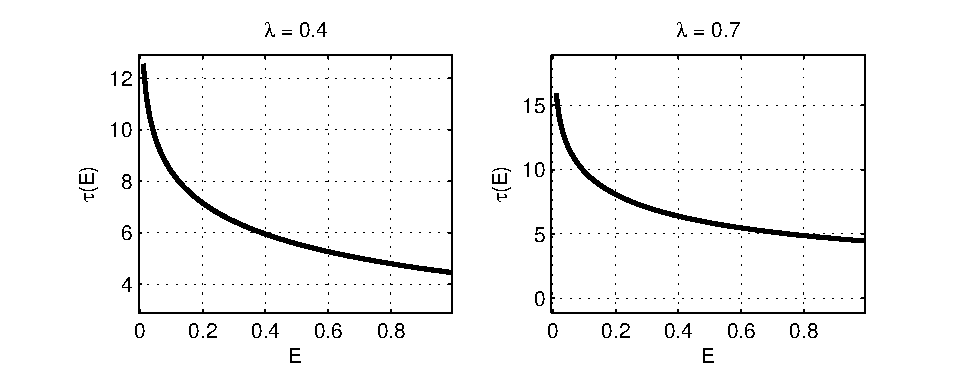
\includegraphics[width=1\linewidth]{pic/tau_on_E_Rabi.eps}}
\caption{$\tau(E)$, Rabi, {\bf qualitative only!}}
\end{figure}
%

\textbf{Квантовый осциллятор.}
Рассмотрим в нуле малые колебания квантового гармонического осциллятора: $\sn~x \sim x$, $\cn~x \sim 1$, $\dn~x \sim 1$.
Уравнение квантового осциллятора
%
\begin{equation}
\frac{d^2 \Psi}{dx^2} + (E - \left( \frac{S \Lambda}{2} \right)^2 x^2) \Psi = 0.
\end{equation}
%
После замены $x \to \sqrt{\frac{S \Lambda}{2}} x$, $\tilde{E} = \frac{2}{S \Lambda} E$:
%
\begin{equation}
\frac{d^2 \Psi}{dx^2} + (\tilde{E} - x^2) \Psi = 0.
\end{equation}
%
Уровни энергии: $\tilde{E} = 2n + 1$ или $E = S \Lambda (n + \frac{1}{2})$.
Собственные функции выражаются через полиномы Эрмита.

\paragraph{Период малых колебаний термона.}
Он связан с температурой фазового перехода.
Рассмотрим малые колебания в яме: $\sn~x \sim x$, $\cn~x \sim 1$, $\dn~x \sim 1$.
Уравнение, описывающее мылые колебания:
%
\begin{equation}
\ddot{x} - 2S^2 (\frac{1}{4} \Lambda^2 - \lambda (1 - \lambda)) x = 0.
\end{equation}
%
Частота малых колебаний:
%
\begin{equation}
\omega_0 = \sqrt{2S^2 (\lambda (1 - \lambda) - \frac{1}{4} \Lambda^2)}.
\end{equation}
%
Период мылых колебаний
%
\begin{equation}
\tau_0 = \frac{2 \pi}{\omega_0} = \frac{2 \pi}{\sqrt{2S^2 (\lambda (1 - \lambda) - \frac{1}{4} \Lambda^2)}}.
\end{equation}
%
Условие, при котором существует симметричная double-well ловушка, поддерживающая существование термона в окрестности точки $x = 0$:
%
\begin{equation}
\lambda (1 - \lambda) > \frac{1}{4} \Lambda^2.
\end{equation}
%

\end{document}